%stpa

\documentclass[../../main/main.tex]{subfiles}


\begin{document}
\title{System-Theoretic Process Analysis}


\chapter{System-Theoretic Process Analysis}
\section{Systems Engineering}
\section{Systems Security Engineering}
\section{System-Theoretic Process Analysis} The primary source for this section is the \glsentryshort{stpa} Handbook \cite{stpa}. It is referred to as the "handbook" in the remainder of this chapter.

System-Theoretic Process Analysis is a systems engineering process that helps the engineer identify and mitigate stakeholder losses. It does this using a four step process that is founded on the System-Theoretic Accident Model and Processes (STAMP).  

STAMP is a way of thinking about how accidents occur.  It assumes both a traditional and a system theoretic view.  In the traditional view, accidents are caused by unsafe chains of events.  In the system theoretic view, accidents are also caused by dynamic and complex interactions. System theory focuses on the system as a whole rather than as a collection of subcomponents.  The need for a system theory approach is epitomized in the notion that the whole is greater than the sum of its parts.  From the complex interactions of individual components arise emergent properties. These properties can be thought of as a higher order that is not predictable from the behavior of the individual components.

Whereas STAMP is a way of thinking about the causes of accidents, STPA is a method to analyze systems in order to prevent or mitigate losses caused by these accidents.  

\section{STPA Overview: Four Steps}
STPA is a four step process.  Figure \ref{4step} diagrams these four steps.  The four steps are briefly described below and then applied to the patrol base operations in the next section.

\begin{figure}[h]
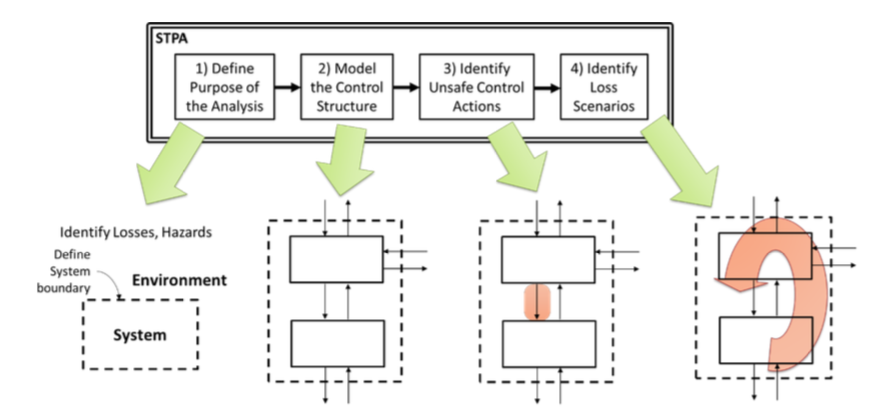
\includegraphics[width=\linewidth]{../figures/4step}
\caption{\label{4step} Four step process of STPA. (Image captured from the \glsentryshort{stpa} Handbook \cite{stpa}.)}
\end{figure}


\paragraph*{Step 1: Define The Purpose of The Analysis}
The first step defines the purpose of the analysis.  It defines the stakeholders and losses from the their perspective.  It also defines the system boundaries, subsystems, environment, inputs, and outputs.  

\paragraph*{Step 2: Model The Control Structure}
The second step models the system.  The model is called a control structure.  It defines the relationships and interactions within the system.

\paragraph*{Step 3: Identify Unsafe Control Actions}
The next step looks links the control actions in the model to the losses described in step 1.

\paragraph*{Step 4: Identify Loss Scenarios}
The last step identifies scenarios that could cause the loss-linked control actions described in step 3.  This analysis should be used to guide system security engineering decisions.


\section{STPA on Patrol Base Operations}
The previous section briefly describes the basic four-step process for STPA.  This section applies that process to the patrol base operations.

\subsection{Step 1: Define The Purpose of The Analysis}
\subsubsection{Define The Purpose of The Analysis}
The purpose of this analysis is to demonstrate the systems security engineering objective (as described by NIST Special Publication 800-160) of designing trustworthy systems with regards to complete mediation.  Complete mediation is the demonstrated outcome of applying the \glsentryshort{csbd} methodology to automated systems.  In this particular analysis, \glsentryshort{csbd} is applied to a non-automated, human-centered system exemplified by the U.S. Ranger Handbook's patrol base operations.  Thus, the more immediate goal is to demonstrate complete mediation in the patrol base operations.  A side-effect is a more thorough understanding of how access-control principals function in non-automated, human-centered military systems.  

\subsubsection{Identify Losses  with Regards to The Stakeholders}
Losses are defined with regards to stakeholders.  These are described below.

\begin{itemize}
\item U.S. Government\\
As a stakeholder, the U.S. Government is very much concerned with national security. Therefore, mission failure is a loss.  In addition, some activities could jeopardize the war fighting effort and national security.  For example, discovery of the patrol base operations could reveal information about the war fighting strategy.  The loss of sensitive technologies either to the enemy or to non-authorized individuals could weaken America's technological superiority.  Therefore, mission discovery and loss of equipment are also losses.  
\item U.S. Army\\
The more immediate stake for the U.S. Army is successfully carrying out the mission.  Again, mission failure is a loss.
\item U.S. Intelligence Community\\
The U.S. intelligence community has a mission to gather intelligence that is critical for national security and mission success.  For reconnaissance missions, mission failure is a loss. For covert missions, discovery of the mission is a loss.  Also, capture of any personnel with sensitive information is a loss. 
\item U.S. military personnel and their families\\
The safety and well-being of military personnel is a concern for all stakeholders.  Nevertheless, it is the most immediate concern of the military personnel themselves.  Therefore, capture, morbidity, and morality are a loss.
\item U.S. Taxpayers\\
The most immediate concern for U.S. taxpayers is the cost war.  Therefore, equipment loss and damage are losses.  
\item U.S. Politicians\\
A concern for all politicians is national security.  Therefore, mission failure is a loss.   But, politicians are elected officials and held accountable by the public for actions taken by the U.S. government.  This means that negative publicity is a loss.  
\item Military Industrial Complex\\
The military industrial complex is a vital asset to national security and plays a critical role in the lives and safety of military personnel as well as United State's military superiority.  They have a stake in demonstrating the superiority of their equipment.  Therefore, equipment failure is a loss.  They also have a stake in demonstrating that their equipment provides U.S. war fighters with an edge in the battlefield.  Therefore, mission failure is a loss.
\item The enemy\\
The enemy has a stake in mission failure.  Their loss is considered a gain.  Therefore, mission failure is a loss.  
\item Regional peoples\\
Regardless of whether the patrol base operations are conducted in a foreign land or at home, preservation of culture, civilian lives, and resources are a concern.  Therefore, disruption of the local culture and damage to resources is a loss. 
\end{itemize}

Thus, from the stakeholders perspective, identified losses are: mission failure; mission discovery; capture, morbidity, and mortality; equipment loss and damage; negative publicity; disruption of local culture and damage to resources.  The labels for these losses are 

\begin{itemize}
\item L-1: Mission failure
\item L-2: Capture, morbidity, and mortality
\item L-3: Mission discovery
\item L-4: Equipment loss or damage
\item L-5: Negative publicity
\item L-6: Disruption of local culture and damage to resources
\end{itemize}

\subsubsection{Define The System Boundaries}
The primary reference for this section is the U.S. Ranger Handbook \cite{rangermanual}.

One way to describe the patrol base operations is with the mission activity specification.  This describes the \textit{what}, \textit{how}, and \textit{why} of the operations. The mission activity specification for the patrol base operations are shown in table \ref{pbtab}

\parskip=8pt
\begin{table}[h!]
\begin{center}
\begin{tabular}{ | m{3.3em} | m{3.8cm}| m{9cm} | } 
\hline
\multicolumn{3}{|c|}{Patrol Base Operations: Mission Activity Specification} \\
\hline \hline
Purpose & A system to & establish a security perimeter when a squad or platoon halts for an extended period of time \\ 
\hline
Method & by means of  & planning, reconnaissance, security, control, and common sense  \\ 
\hline
Goal & in order to & 
\begin{itemize}
\item avoid detection
\item hide a unit during a long, detailed reconnaissance
\item perform maintenance on weapons, equipment, eat, and rest
\item plan and issue orders
\item reorganize after infiltrating an enemy area
\item establish a base from which to execute several consecutive or concurrent operations
\end{itemize}
\\ 
\hline
\end{tabular}
\end{center}
\caption{Mission Activity Specification for Patrol Base Operations.  Adapted from the U.S. Army Ranger Handbook 2017 (7-46) \cite{rangermanual}.}
\label{pbtab}
\end{table}
\parskip=18pt

The mission activity specificity highlights one of the challenges in modeling the patrol base operations: it's generality.  To put this into perspective, the patrol base may execute operations such as engaging the enemy or conducting reconnaissance.  Or, it may be a temporary rest and recovery position.  A patrol engaged in patrol base operations may consist of a fire team comprised of ? soldiers, a platoon comprised of ? soldiers, or something in-between. 

Without loss of generality, the patrol base operations are defined in terms of the system, system boundaries, subsystems, environment, input, and outputs.  Figure \ref{system} shows a diagram relating a system to its boundaries, subsystems, and inputs and outputs.  These are described below.

\begin{figure}[h]
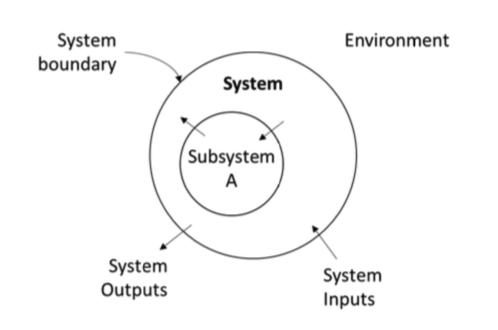
\includegraphics[width=\linewidth]{../figures/system}
\caption{\label{system} Relationship of system to system boundaries, subsystems, inputs, and outputs. (Image captured from the \glsentryshort{stpa} Handbook \cite{stpa}.)}
\end{figure}
\paragraph*{System}
In this master thesis, the "system" refers to a platoon-sized patrol base operation.  This is the best choice because a platoon-sized operation may be scaled-down to accommodate a squad-sized or fire team-sized detachment, but not the other way around. 

\paragraph*{System Boundaries}
The mission details are intentionally kept vague to accommodate as many types of missions as possible.  The system boundaries for the model are the start and end of the mission\footnote{Note that the Ranger Handbook specifically states that "because a patrol is an organization, not a mission, it is not correct to speak of giving a unit a mission to "patrol.""  The term "mission" used in this master thesis refers generally to the mission (or objectives) of the patrol base operations, and does not refer to the patrol as being a mission.}. In this master thesis, the patrol base operations begin in the planning phase when the patrol leader receives the mission.  The patrol base operations end after the patrol withdraws from the operations and returns to the main body\footnote{Completion should include reporting to the commander.  However, for the purposes of this master thesis, it was sufficient to conclude a withdraw.  Nevertheless, with our model of the patrol base operations, it is easy to add a phase for reporting to the commander.}

\paragraph*{Subsystem}
A subsystem in the patrol base operations is any smaller group of soldier assigned to a specific task such as security or reconnaissance.  This may include a squad or fire team.  

\paragraph*{Environment}
The mission is determined by the greater-wisdom of the U.S. Army leadership at the time of need.  This means that environmental boundaries, mission boundaries, and other system requirements must be determined by the patrol leader  (referred to as the platoon leader in subsequent chapters) after the mission is received and during the planning phase.  For this reason, STPA analysis should be performed on a mission before it is referred to the patrol.  But also, patrol leaders should be trained in STPA to make a quick and accurate analysis of mission-specific system boundaries.  


\paragraph*{System Inputs and Outputs}
The system input is the mission handed down by the U.S. Army leadership.  Additional inputs such as equipment, weapons, and additional personnel are determined when the mission is received. 

System outputs are mission dependent.  They may be successful engagement with the enemy, the capture of an enemy combatant, acquisition of specific intelligence, or anything else defined by the mission objectives.

\subsubsection{Identify System-level Hazards}
System-level hazards are unsafe states of the system that will lead to loss in a worst-case scenario.  System-level hazards are either preventable or mitigable.

STPA links these hazards to one or more losses.  A list of system-level hazards with explanations for the patrol base operations is described below.

\begin{itemize}
\item H-1: Soldier is captured, injured, and killed [L-1, L-2, L-3, L-5].\\
Capture, injury, and loss of life could cause mission failure.  A captured soldier draws unwanted attention to the patrol base operations and poses a security threat.  An injured soldier or casualty must be cared for.  These scenarios all require a reprioritization of the mission to mitigate the loss.  Capture and loss of life, in particular, can generate negative publicity for the war fighting effort. 

\item H-2: Patrol base attracts unwanted attention [L-1, L-3, L5].\\
If the patrol base is conducted in secret, then any contact with the enemy or locals is unwanted.  This means that the mission has been compromised.  Furthermore, it is more-and-more likely in the age of Facebook and Twitter that contact with locals will be reported.  This could cause negative publicity for the war effort. 

\item H-3: Mission is not properly communicated and understood [L-1, L-2, L-3, L-5, L-6].\\
The objectives of the mission must be clearly communicated in oder to be carried out.  In worst-case scenarios, the misinformed soldiers could come into contact with the enemy, causing capture, injury, or death.  A wrong mission, or a right mission at the wrong location, could have the wrong intelligence.  This could also disrupt the local population and resources.

\item H-4: Mission is changed [L-1].\\
A change of mission effectively cancels the current mission. This could be perceived as failure depending on the reason for the cancellation.

\item H-5: Operational protocols not followed properly [L-1, L-2, L-3, L-4, L-5, L-6].\\
The patrol base operations are described in sufficient detail because they have been refined over many years to provide U.S. Army Rangers with the best chances of success.  They should be followed.  In worst-case scenario, not following protocols could cause the mission to fail, capture, injury, and death, mission discovery, equipment loss or damage, and disruption of the local population and resources.  All of these cases could cause bad publicity.

\item H-6: Team not trained or properly equipped [L-1, L-2].\\
In the worst case scenario, lack of training or improper equipment could cause capture, injury, or death.  It could also cause the mission to fail or be discovered.  In addition, equipment could be lost or damaged and the local population and resources could be disturbed.  All of these could cause negative publicity.

\item H-7: Equipment left behind [L-1,L-3, L-4, L-5, L-6].\\
If equipment is left behind, it could reveal the presence and/or purpose of the patrol base operations.  Sensitive equipment in the wrong hands could weaken the technological superiority of the U.S.. If the lost equipment becomes a feature on social media, this could cause bad publicity for the war fighting effort.  Land mines and other dangerous equipment could affect local people and make resources (such as land) unusable.

\item H-8: Equipment malfunction, not used properly, or properly maintained [L-4].\\
\end{itemize}

\subsubsection{Define System-level Constraints}
System-level constraints are designed to prevent or mitigate hazards.  These are defined below for each hazard.

\begin{itemize}
\item SC-1: Soldiers should avoid being captured, injured, or killed [H-1].
\item SC-2: If not engaging the enemy, patrol base operations must avoid contact with enemy or locals [H-2].
\item SC-3: If engaging the enemy, patrol base operations must be kept secret until contact with enemy [H-1, H-2].
\item SC-4: Patrol base operations must not leave any equipment, trash, personal belongs, or other indicators of their presence [H-2, H-7].
\item SC-5: Patrol base must receive mission, verify mission receipt, and restate mission [H-3].
\item SC-6: Unless otherwise ordered, patrol base must maintain communication with main body to listen for a change of mission [H-3, H-4].
\item SC-7 Soldiers must follow proper protocols [H-6].
\item SC-8: Soldiers must be trained on all procedures and equipment required to successful accomplish objectives [H-6].
\item SC-9: Soldiers must be informed of their responsibilities within the patrol base and of the chain of command [H-6].
\item SC-10: Soldiers should properly use and maintain equipment [H-6, H-8].
\end{itemize}

\subsubsection{Refine System-level Hazards}
It is optional to refine system-level hazards.  

\begin{itemize}
\item H-1: Soldier is captured, injured, and killed [L-1, L-2, L-3, L-5].\\
\begin{itemize}
\item Captured

\begin{itemize}
\item H-1.1: Soldier with intelligence specific to mission is captured.
\item H-1.2: Soldier with intelligence specific to other missions is captured.
\item H-1.3: Soldier with intelligence critical to national security is captured.
\item H-1.4: Soldier is captured by terrorist.
\item H-1.5: Soldier is captured by enemy who will observe Geneva Conventions.
\end{itemize}

\item Injured
\begin{itemize}
\item H-1.6: Soldier has mild injured that must be treated after mission, but can continue with mission.
\item H-1.7: Soldier is injured, cannot participate in mission, but can wait for mission to complete.
\item H-1.8: Soldier is injured, requires immediate medical attention, must return to base, and requires assistance.
\end{itemize}

\item Killed
\begin{itemize}
\item H-1.9: Soldier is killed by enemy contact.
\item H-1.10: Soldier is killed by some other hazard.
\item H-1.11: Soldier is missing in action and presume killed.
\end{itemize}
\end{itemize}

\item H-2: Patrol base attracts unwanted attention [L-1, L-3, L5].\\

\begin{itemize}
\item H-2.1: Patrol base attracts unwanted attention from local population.
\item H-2.2: Patrol base attracts unwanted attention from enemy.
\end{itemize}

\item H-3: Mission is not properly communicated and understood [L-1, L-2, L-3, L-5, L-6].\\
\begin{itemize}
\item H-3.1: Mission not received.
\item H-3.2: Mission not understood.
\end{itemize}


\item H-4: Mission is changed [L-1].\\

\item H-5: Operational protocols not followed properly [L-1, L-2, L-3, L-4, L-5, L-6].\\
\begin{itemize}
\item H-5.1: Chain of command not followed.
\item H-5.2: Military doctrine not followed.
\item H-5.3: Patrol base operational procedures not followed.
\item H-5.4: Geneva Convention not followed.
\end{itemize}

\item H-6: Team not trained or properly equipped [L-1, L-2].\\
\begin{itemize}
\item H-6.1: Team not properly trained on military procedures.
\item H-6.2: Team not trained properly on specific mission.
\item H-6.3: Team not trained properly on mission-specific equipment.
\item H-6.4: Team not trained on order of succession within patrol base.
\end{itemize}


\item H-7: Equipment left behind [L-1,L-3, L-4, L-5, L-6].\\
\begin{itemize}
\item H-7.1: Trash and other items left behind.
\item H-7.2: Weapons left behind.
\item H-7.3: Sensitive technologies left behind.
\end{itemize}

\item H-8: Equipment malfunction, not used properly, or properly maintained [L-4].\\
\begin{itemize}
\item H-8.1: Equipment malfunction.
\item H-8.2: Equipment not used properly causing malfunction.
\item H-8.3: Equipment not maintained properly causing malfunction.
\end{itemize}


\end{itemize}

\subsubsection{Refine System-level Constraints}
System-level constraints can be redefined as well.  For this particular project, too much detail is not helpful because the master thesis is designed to test the feasibility of applying the \glsentryshort{csbd}.  This means that a detailed STPA of the patrol base operations is beyond scope.  Nevertheless, it is possible to demonstrate this part of the STPA to get a feel for it.


Patrol base operations cover a variety of operational objectives.  The U.S. Army Ranger Handbook describes : Reconnaissance, Combat, Ambush, Raid, Supporting, Movement To Contact, already has a description of the types of mission (i.e., rest and resupply, reconnaissance, engage enemy) and specific plans for these mission.  Consideration of all these types of missions is beyond the scope of this master thesis. A complete STPA on the patrol base operations would involve consideration of each type of mission.  It would also include how the input is handled by the higher-up leadership.  Within scope, it is sufficient to note that many details of how the operations will be worked out by the leadership in advance of the mission.  This includes standard and specialized training.  

The mission is handed down to the patrol leader at the start of the mission the patrol base operations. This is the input to this system.  The patrol leaders must plan according to this input. Within the system, system-level constraints are mission-specific. Nevertheless, it is possible to refine the system-level constraints broadly or to at least recognize that these are considerations made after receipt of the mission. Some system-level constraints are shown in table \ref{slconstraints} and categorized based on hazards.

\parskip=8pt

\begin{longtable}[h]{ | m{7.5cm} |  m{7.5cm} | } 

\hline \hline
 \multicolumn{2}{| c |}{System-level Hazards and Constraints}\\
\hline \hline
Refined Hazard & Refined Constraint\\
\hline \hline
 \endfirsthead


\hline \hline
 \multicolumn{2}{| c |}{System-level Hazards and Constraints}\\
\hline \hline
Refined Hazard & Refined Constraint\\
\hline \hline
\endhead

\hline
\multicolumn{2}{|c|}{H-1: Soldier is captured, injured, and killed [L-1, L-2, L-3, L-5]}\\
\hline
H-1.1: Soldier with intelligence specific to mission is captured. 
& 
SC-1.1: Upon receiving the mission, patrol leaders should assess likelihood of capture and how to respond.\\ 
\hline
H-1.2: Soldier with intelligence specific to other missions is captured.
& 
SC-1.2: Considerations should be made prior to the mission as the whether these soldiers should be assigned to the patrol.Upon receiving the mission, patrol leaders should assess likelihood of capture and how to respond.   \\ 
\hline
H-1.3: Soldier with intelligence critical to national security is captured.
& 
SC-1.3: Considerations should be made prior to the mission as the whether these soldiers should be assigned to the patrol. Upon receiving the mission, patrol leaders should assess likelihood of capture and how to respond.  \\ 
\hline
H-1.4: Soldier is captured and will probably be killed.  
& 
SC-1.4: Upon receiving the mission, patrol leaders should assess how to respond (i.e., halt mission and rescue soldier?  Halt mission? Etc.).  \\ 
\hline
H-1.5: Soldier is captured by enemy who will observe Geneva Conventions.
& 
SC-1.5: Upon receiving the mission, patrol leaders should assess how to respond (i.e., halt mission and rescue soldier?  Halt mission? Etc.).  \\ 
\hline
H-1.6: Soldier has mild injury that must be treated after mission, but can continue with mission.
& 
SC-1.6: But, in most situations, Soldier/Medic renders medical aid and Soldier can tough-it-out.  Mission continues.  \\ 
\hline
H-1.7: Soldier is injured, cannot participate in mission, but can wait for mission to complete.
& 
SC-1.7: Soldier should be treated and leaders should assess if mission can continue without soldier.  \\ 
\hline
H-1.8: Soldier is injured, requires immediate medical attention, must return to main body, and requires assistance.
& 
SC-1.8: Depending on the mission, Leader assess if mission can continue.  Injured soldier is brought to main body.  \\ 
\hline
H-1.9: Soldier is killed by enemy contact.
& 
SC-1.9: Depending on the mission, Leader assess if mission can continue.  For example, is engagement with enemy part of the mission?  If so, continue mission?  If mission does not include contact with enemyIf mission continues, Leader should asses how to handle body until mission completion.    \\ 
\hline
H-1.10: Soldier is killed by some other hazard.
& 
SC-1.10  \\ 
\hline
H-1.11: Soldier is missing in action and presume killed.
& 
SC-1.11  \\ 

\hline
\multicolumn{2}{|c|}{H-2: Patrol base attracts unwanted attention [L-1, L-3, L5].}\\
\hline
H-2: Patrol base attracts unwanted attention [L-1, L-3, L5].
& 
SC-2.1  \\ 
\hline
H-2.1: Patrol base attracts unwanted attention from local population.
& 
SC-2.1  \\ 
\hline
H-2.2: Patrol base attracts unwanted attention from enemy.
& 
SC-2.2  \\ 


\hline
\multicolumn{2}{|c|}{H-3: Mission is not properly communicated and understood [L-1, L-2, L-3, L-5, L-6].}\\
\hline
H-3.1: Mission not received.
& 
SC-3.1 \\
\hline
H-3.2: Mission not understood.
& 
SC-3.2 \\

\hline
\multicolumn{2}{|c|}{H-4: Mission is changed [L-1].}\\
\hline
H-4: Mission is changed [L-1].
& 
SC-4\\

\hline
\multicolumn{2}{|c|}{H-5: Operational protocols not followed properly [L-1, L-2, L-3, L-4, L-5, L-6].}\\
\hline
 H-5.1: Chain of command not followed.
 & 
SC-5.1\\
\hline
H-5.2: Military doctrine not followed.
 & 
SC-5.2\\
\hline
H-5.3: Patrol base operational procedures not followed.
 & 
SC-5.3\\
\hline
H-5.4: Geneva Convention not followed.
 & 
SC-5.4\\
\hline
H-5.5: Intra-patrol miscommunication.
 & 
SC-5.4\\

\hline
\multicolumn{2}{|c|}{H-6: Team not trained or properly equipped [L-1, L-2].}\\
\hline
H-6.1: Team not properly trained on military procedures.
 & 
SC-6.1\\
\hline
H-6.2: Team not trained properly on specific mission.
 & 
SC-6.2\\
\hline
H-6.3: Team not trained properly on mission-specific equipment.
 & 
SC-6.3\\
\hline
H-6.4: Team not trained on order of succession within patrol base.
 & 
SC-6.4\\

\hline
\multicolumn{2}{|c|}{H-7: Equipment left behind [L-1,L-3, L-4, L-5, L-6].}\\
\hline
H-7.1: Trash and other items left behind.
 & 
SC-7.1\\
\hline
H-7.2: Weapons left behind.
 & 
SC-7.2\\
\hline
H-7.3: Sensitive technologies left behind.
 & 
SC-7.3\\

\hline
\multicolumn{2}{|c|}{H-8: Equipment malfunction, not used properly, or properly maintained [L-4].}\\
\hline
H-8.1: Equipment malfunction.
 & 
SC-8.1\\
\hline
H-8.2: Equipment not used properly causing malfunction.
 & 
SC-8.2\\
\hline
H-8.3: Equipment not maintained properly causing malfunction.
 & 
SC-8.3\\
\hline

\caption{Refined system-level hazards and derived system-level constraints.  Adapted from the U.S. Army Ranger Handbook 2017 (7-46) \cite{rangermanual}\label{slconstraints}.}\\

\end{longtable}
\parskip=18pt


\subsection{Step 2: Model The Control Structure}


\subsection{Step 3: Identify Unsafe Control Actions}
\subsection{Step 4: Identify Loss Scenarios}

\section{Discussion of The Analysis}
\subsection{Recommendations for STPA on Other Military Activities}
\end{document}